\documentclass[
  tikz, convert={density=800, size = 2400x2400},
  border=0.5cm
]{standalone}
\usepackage{amsmath, amssymb, amsthm, bm, bbm, xcolor, tikz}

\usetikzlibrary{shapes.geometric, positioning}
\usetikzlibrary{quotes, angles, calc, backgrounds}

\definecolor{myColor1}{RGB}{153,153,153}
\definecolor{myColor2}{RGB}{230,159,0}
\definecolor{myColor3}{RGB}{86,180,233}
\definecolor{myColor4}{RGB}{0,158,115}
\definecolor{myColor5}{RGB}{240,228,66}
\definecolor{myColor6}{RGB}{0,114,178}
\definecolor{myColor7}{RGB}{213,94,0}
\definecolor{myColor8}{RGB}{204,121,167}

\tikzset{decisionNode/.style={inner sep=7pt, shape=circle,align=center,font=\Huge,draw, fill=gray!40}}
\tikzset{leafNode/.style={inner sep=7pt, shape=circle, align=center, font = \Huge, draw, fill=white}}
\tikzset{decisionRule/.style={shape=rectangle, align=center, font = \normalsize, draw=none, fill=white}}
\tikzset{jump/.style={shape=rectangle, align=center, font=\Large, draw=none, fill=white}}
\tikzset{annotation/.style={shape=rectangle, align=center, font=\Large, draw=none, fill=white}}

\begin{document}
\def\P{\mathbb{P}}

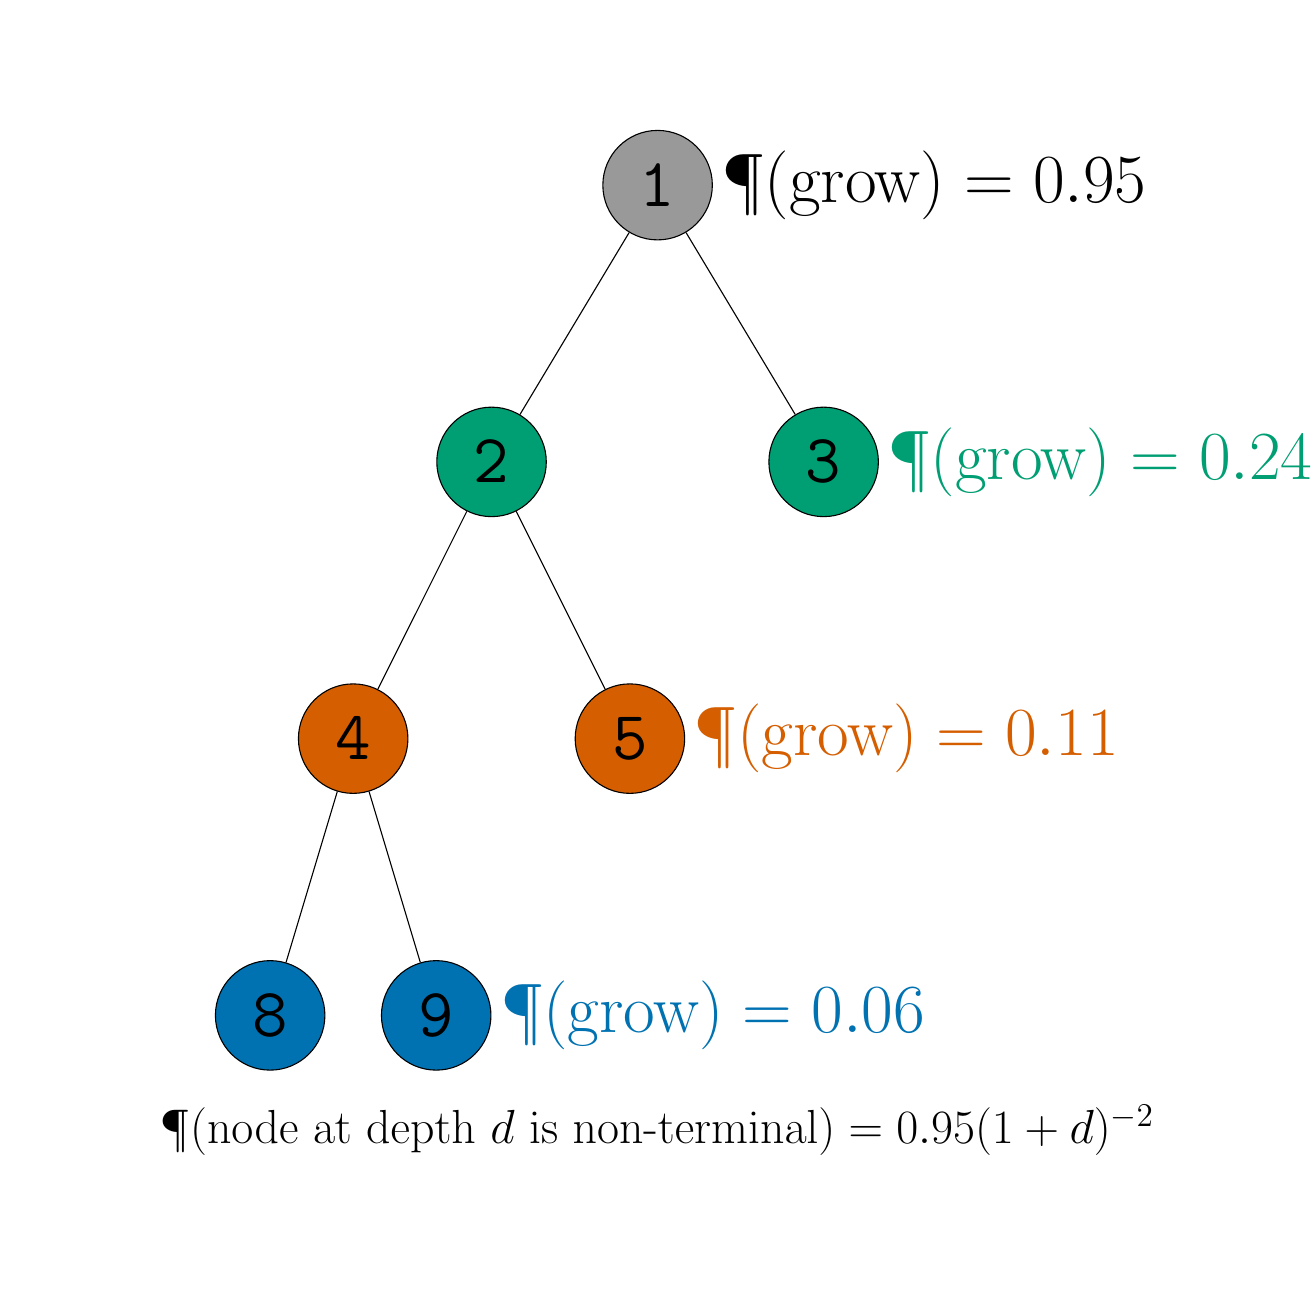
\begin{tikzpicture}[
  background rectangle/.style={fill=white}, show background rectangle,
  level 1/.style={sibling distance = 12em},
  level 2/.style={sibling distance = 10em},
  level 3/.style={sibling distance = 6em},
  level 4/.style={sibling distance = 5em},
  level distance = 10em]

\useasboundingbox (-8,-8) rectangle (8,8);

\node[decisionNode, fill=myColor1, label=right:{\Huge $\P(\text{grow}) = 0.95$}]  (1) at (0,6) {\texttt{1}}
  child{ % 2 and its children
    node[decisionNode, fill=myColor4] (2) {\texttt{2}}
      child{ % 4 and its children
        node[decisionNode, fill=myColor7] (4) {\texttt{4}}
          child{ node[leafNode, fill=myColor6] (8) {\texttt{8}}}
          child{ node[leafNode, fill=myColor6, label=right:{\Huge \textcolor{myColor6}{$\P(\text{grow}) = 0.06$}}] (9) {\texttt{9}} }
      }
      child{
        node[decisionNode, fill=myColor7, label=right:{\Huge \textcolor{myColor7}{$\P(\text{grow}) = 0.11$}}] (5) {\texttt{5}}}
  }
  child{ 
    node[decisionNode, fill=myColor4, label=right:{\Huge \textcolor{myColor4}{$\P(\text{grow}) = 0.24$}}] (3) {\texttt{3}}
  }
;

\node[annotation] at (0, -6) {\LARGE $\P(\text{node at depth $d$ is non-terminal}) = 0.95(1 + d)^{-2}$};

\end{tikzpicture}

\end{document}